\documentclass{article}
\usepackage{caption}
\usepackage{setspace}
\usepackage{amsmath}
\usepackage{amssymb}
\usepackage{amsthm}
\usepackage{empheq}
\usepackage{graphicx}
\usepackage{multirow}
\usepackage{geometry}
\usepackage{listings}
\lstset{frame=tb,
  language=Python,
  aboveskip=3mm,
  belowskip=3mm,
  showstringspaces=false,
  columns=flexible,
  basicstyle={\small\ttfamily},
  numbers=none,
  numberstyle=\tiny\color{gray},
  keywordstyle=\color{blue},
  commentstyle=\color{dkgreen},
  stringstyle=\color{mauve},
  breaklines=true,
  breakatwhitespace=true,
  tabsize=3
}
\usepackage{subfigure}
\usepackage{float}
\usepackage{color}
\usepackage{url}
\usepackage{pgfplots}
\pgfplotsset{compat=1.18}
\definecolor{dkgreen}{rgb}{0,0.6,0}
\definecolor{gray}{rgb}{0.5,0.5,0.5}
\definecolor{mauve}{rgb}{0.58,0,0.82}
% \usepackage{ctex}
\usepackage[ruled,linesnumbered]{algorithm2e}
\usepackage{fontspec}
\setmainfont{Times New Roman}
\geometry{a4paper}
\setlength{\parindent}{2em}


\begin{document}
\title{\vspace{-3cm}\textbf{AMA564 Deep Learning Assignment 2}}
\author{Chen Yushuo\\24081349G}
\maketitle
\subsection*{Question 1}
\subsubsection*{(1).}
For $f_1$, the out put matrix will be $5\times 5$ size. And 
\[y_{11} = 1\times 0 + 1\times 0 +0\times 0+0\times 1 = 0.\]
Repeat it for every entries of $y$, then we can get the result matrix:
\begin{align*}
  y^1 = \begin{bmatrix}
    0&0&0&0&0\\
    1&1&0&1&1\\
    1&1&0&1&1\\
    0&0&0&0&0\\
    1&2&2&2&1
  \end{bmatrix}.
\end{align*}

For $f_2$, the result is:
\begin{align*}
  y^2 = \begin{bmatrix}
    0&1&0&0&1\\
    0&2&0&0&2\\
    0&1&0&0&1\\
    0&1&1&1&1\\
    0&1&1&1&1
  \end{bmatrix}.
\end{align*}

For $f_3$, the result is:
\begin{align*}
  y^3 = \begin{bmatrix}
    0&-1&0&0&-1\\
    -1&0&0&-1&0\\
    -1&1&0&-1&1\\
    0&-1&-1&-1&-1\\
    -1&0&0&0&1
  \end{bmatrix}.
\end{align*}

\subsubsection*{(2).}
{\it MaxPool} will extract the max entry from the $2\times 2$ sub-matrix.
And the final result will be in $3\times 3$ since stride 2.
The result is:
\begin{align*}
  \begin{bmatrix}
    1&0&1\\
    1&0&1\\
    1&1&1
  \end{bmatrix}.
\end{align*}

\subsubsection*{(3).}
If we take the average, all entries will be $(1+1)/9 = 2/9$.
So the result will be:
\begin{align*}
  \begin{bmatrix}
    2/9&2/9\\
    2/9&2/9
  \end{bmatrix}.
\end{align*}

\newpage
\subsection*{Quetion 2.(1).}
\begin{figure}[htbp]
  \centering
  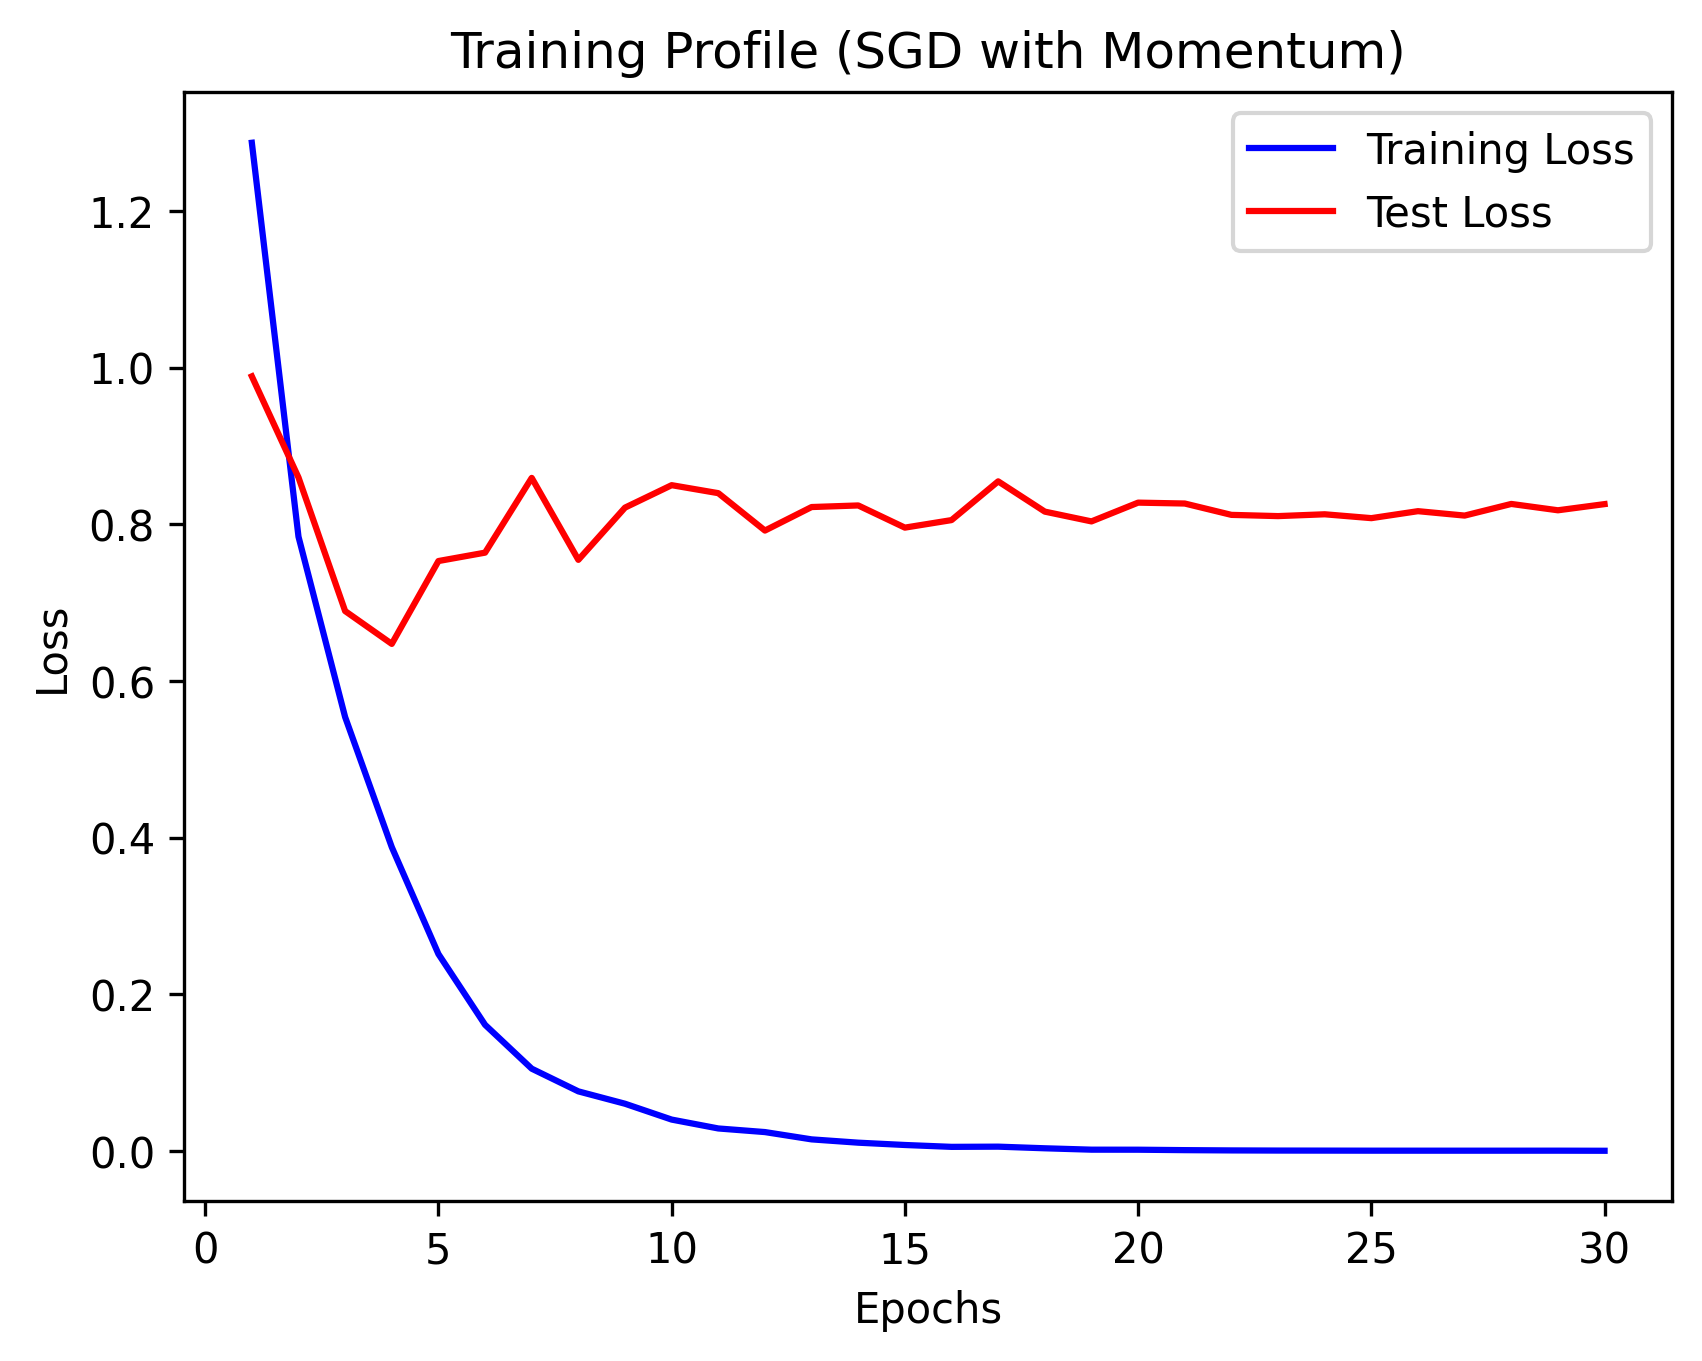
\includegraphics[scale=0.7]{pic/loss_curve_SGD.png}
  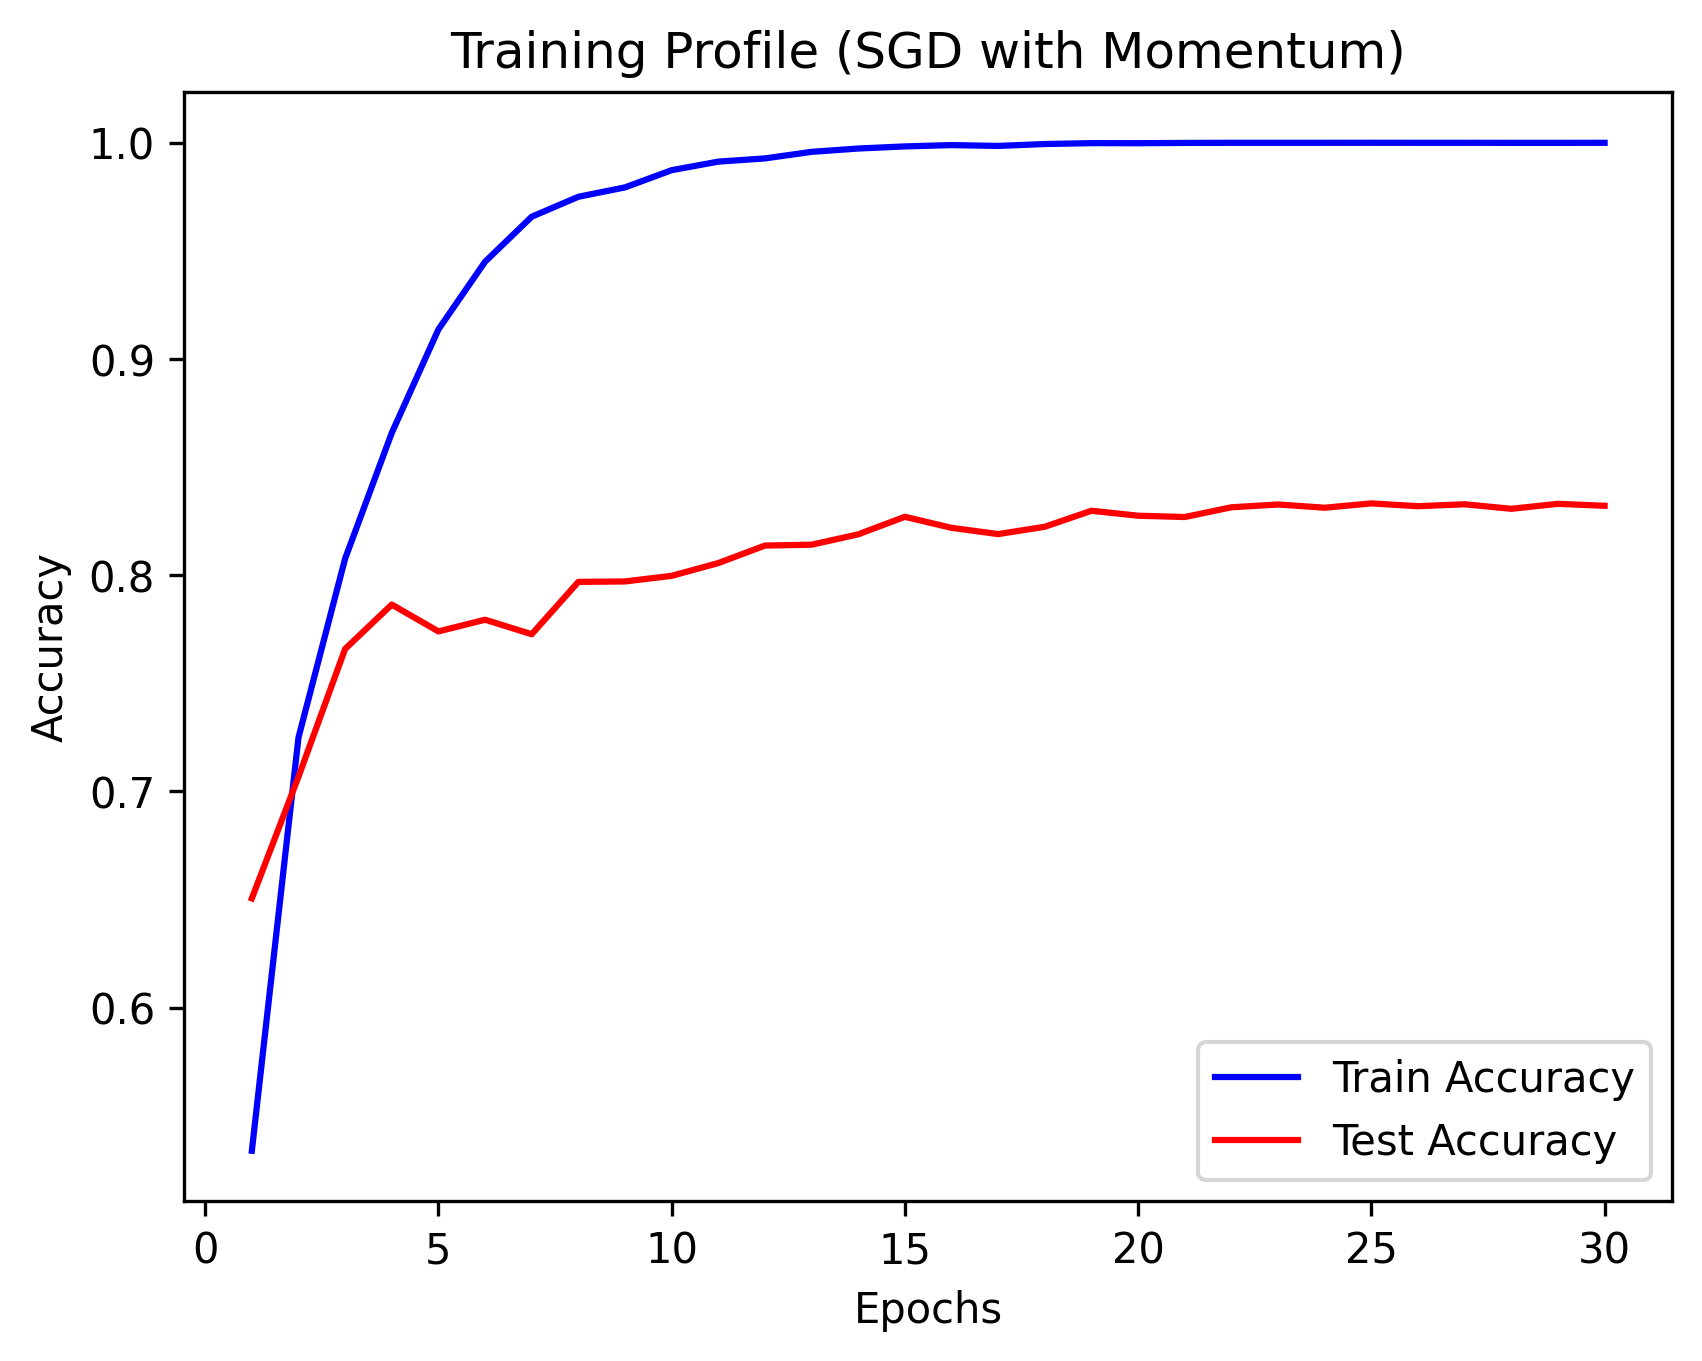
\includegraphics[scale=0.7]{pic/accuracy_curve_SGD.png}
\end{figure}
Train accuracy almost reaches 100\%.
Test accuracy reaches 83\%, avg loss is 0.82 more or less.

\newpage
\subsubsection*{(2).}
\begin{figure}[htbp]
  \centering
  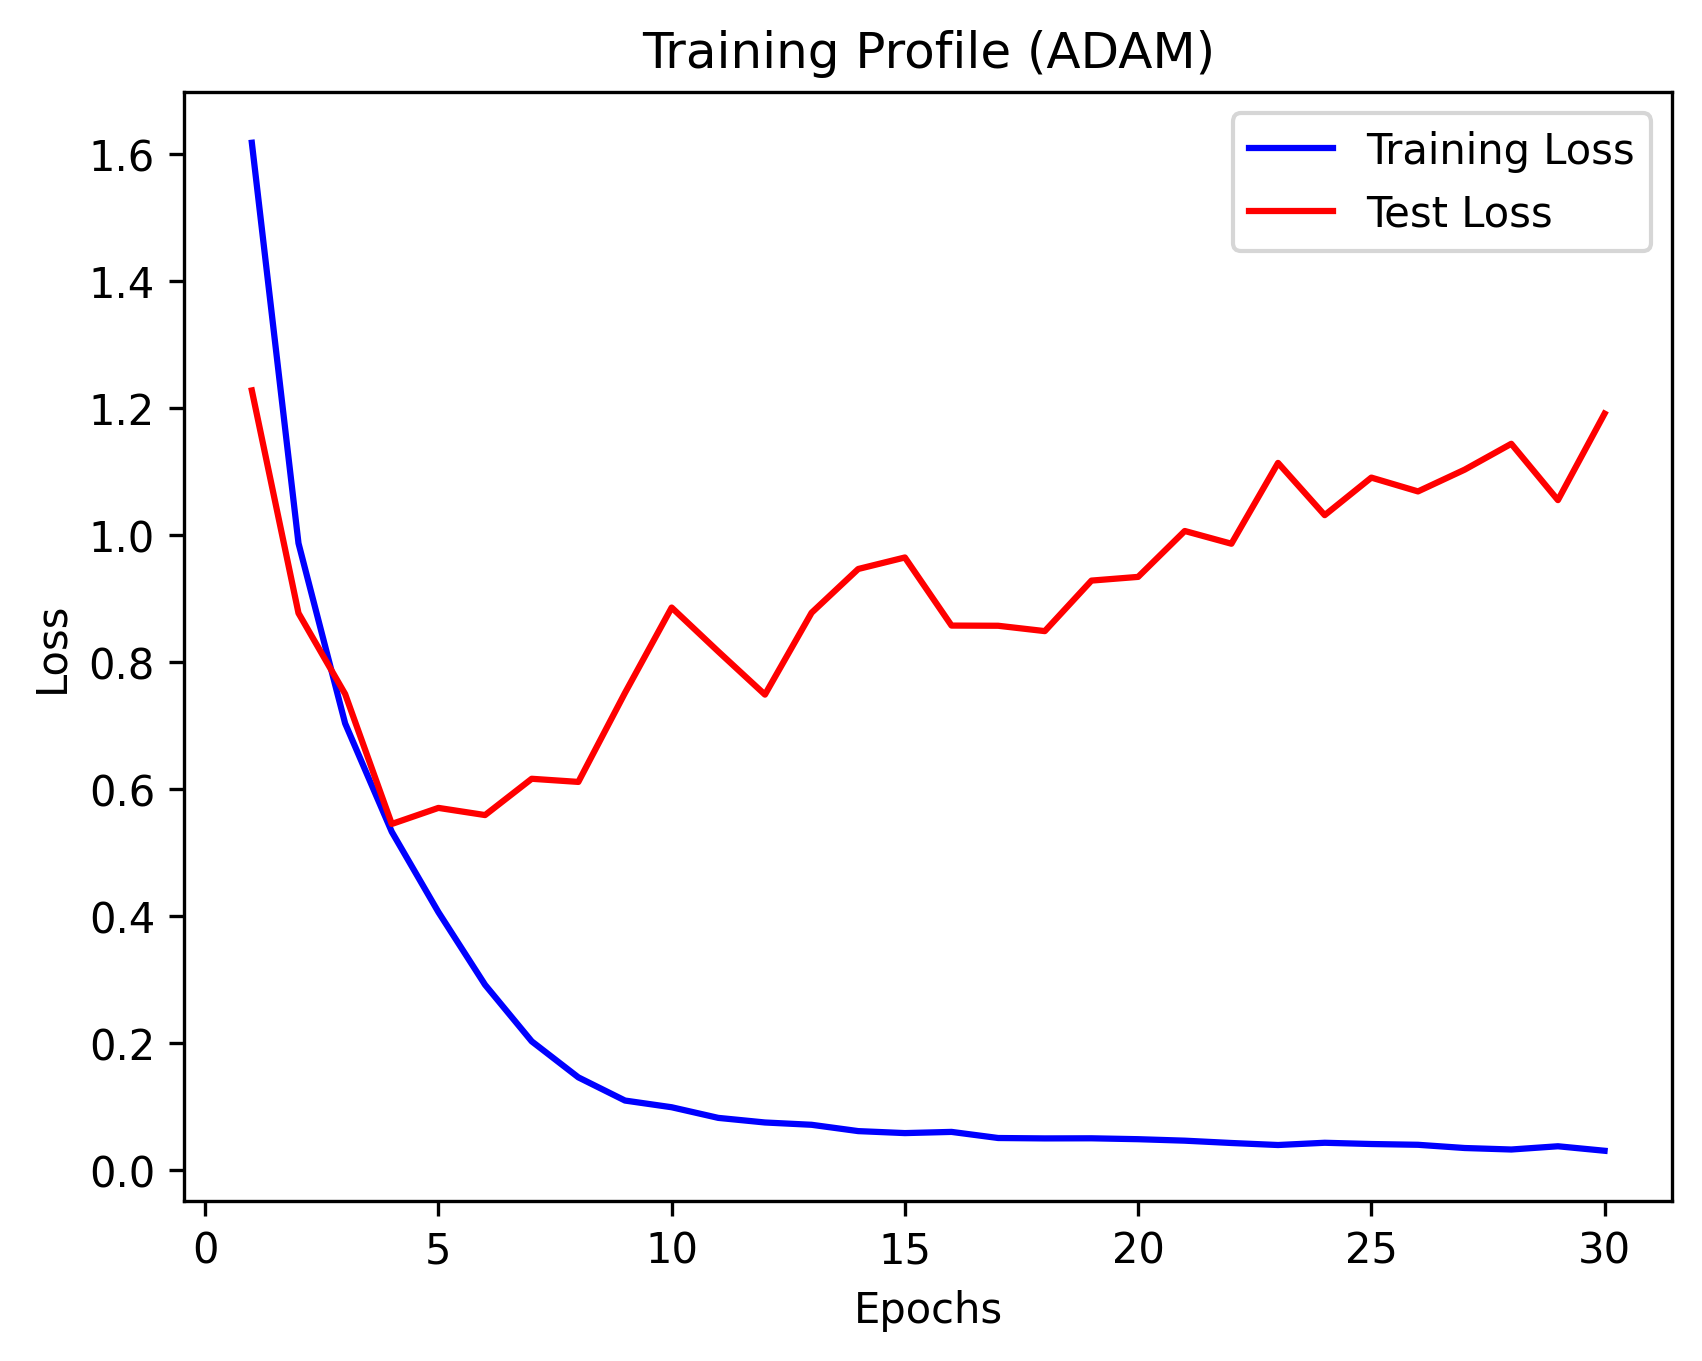
\includegraphics[scale=0.7]{pic/loss_curve_ADAM.png}
  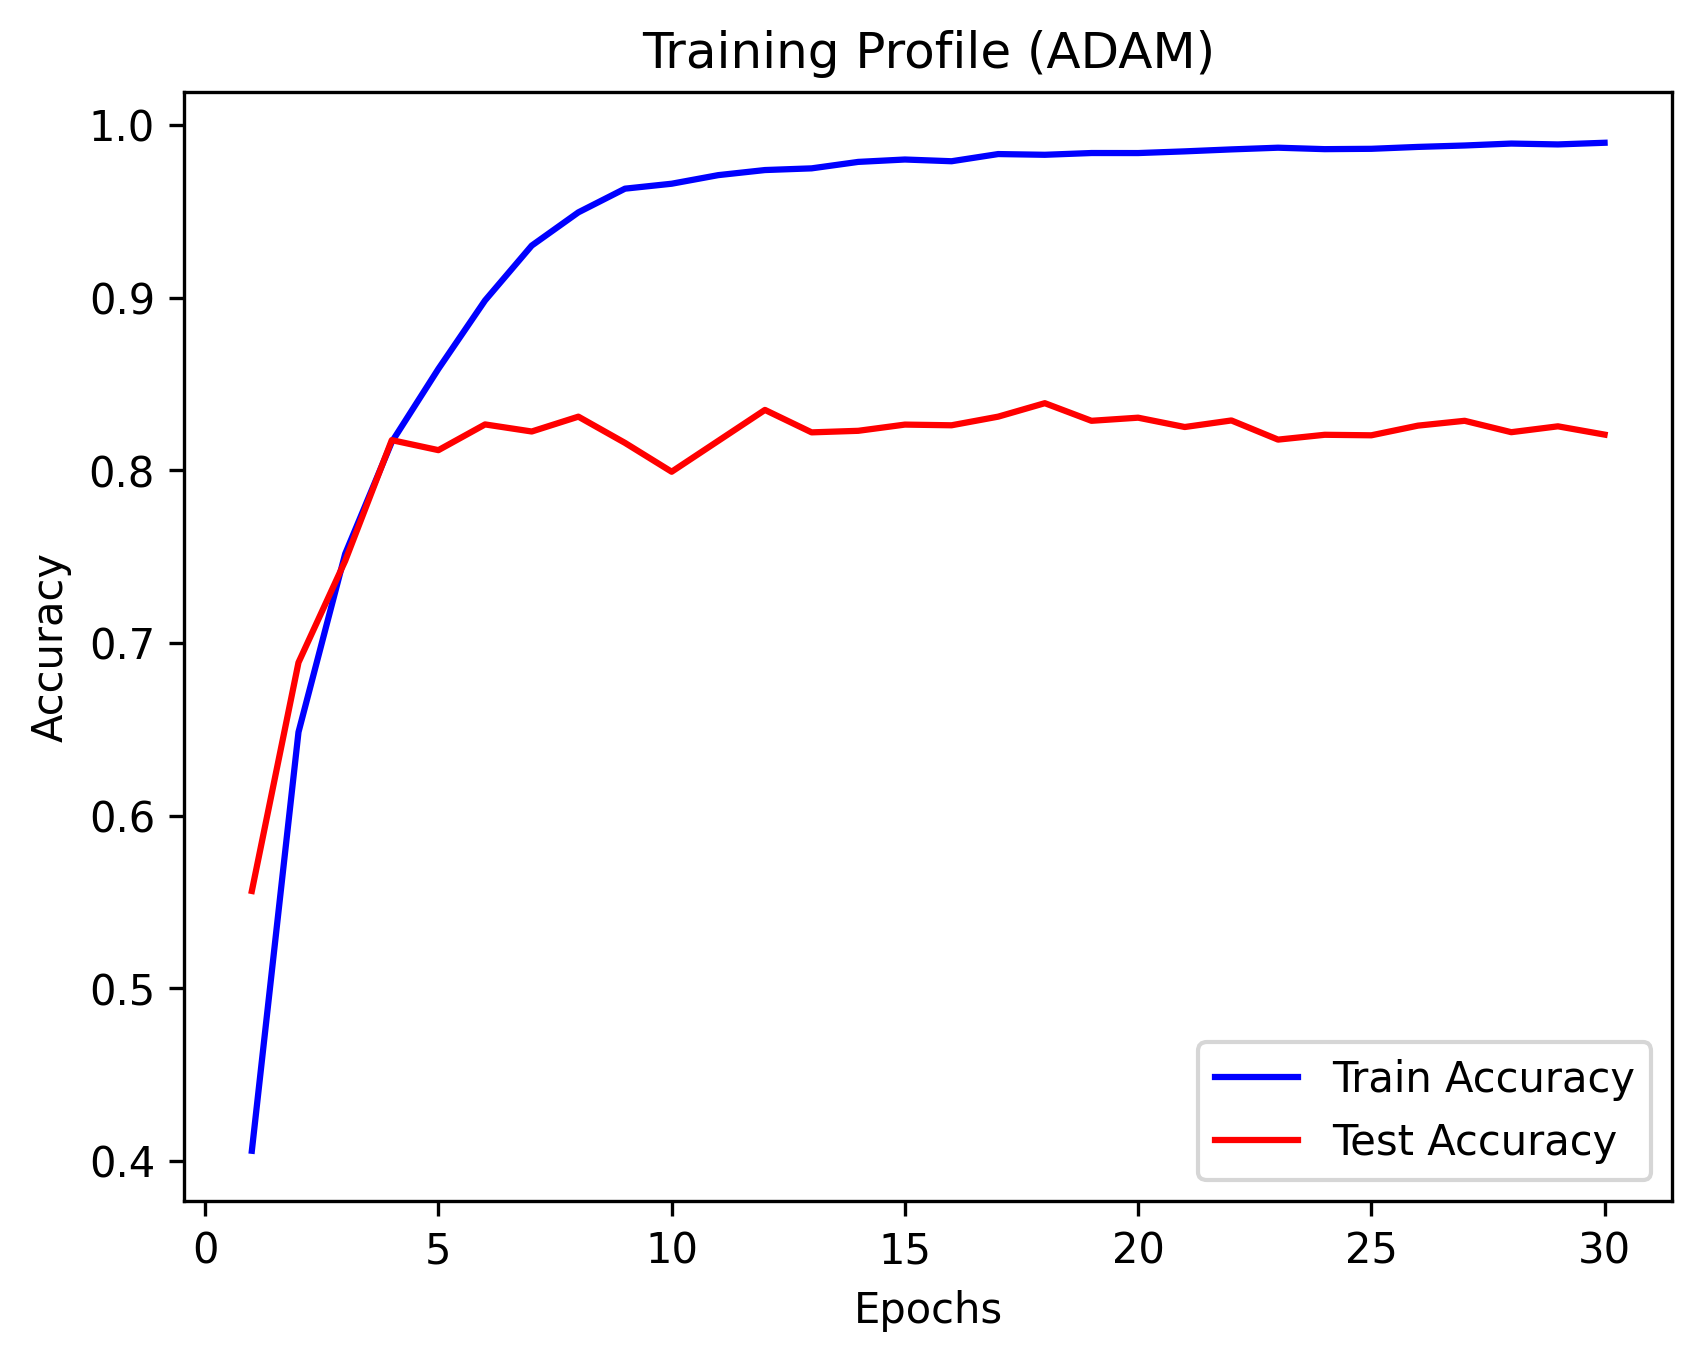
\includegraphics[scale=0.7]{pic/accuracy_curve_ADAM.png}
\end{figure}
Train accuracy also reaches 100\%.
Test accuracy reaches 82.5\%, avg loss is more than 1.15.

\newpage
\subsection*{Question 3.}
(a) False.\\
(b) True.\\
(c) True.\\
(d) False.\\
(e) True.

\subsection*{Question 4.}
(a) - (e):\\
D B B D A.
\end{document}